\section{Introduction}\label{sec:intro}

\subsection{Testing 3\% of a DRP using HSC PDR2}

In preparation for annual DRP (Data Release Processing) campaigns, 
a set of some 17K exposures from the HSC PDR2 dataset were pushed through
a current version of the DRP pipelines.

These exposures are then coadded into 710 tracts, including about 671
WIDE tracts of repeated depth a few in grizy bands, and 39 DEEP+UDEEP 
tracts with up to 426 overlapping exposures in some bands in some UDEEP tracts.
The DEEP+UDEEP tracts covered about 100 square degrees in area, while the
WIDE tracts covered about 1000 square degree to varying depth.

Figure \ref{fig:footprint1} shows the HSC PDR2 footprint processed in equatorial coordinates
on the sky.    A close up of region surrounding the COSMOS UDEEP tracts is shown in Figure \ref{fig:hscmaptract} using the hscMap tool from NAOJ \url{https://hscmap.mtk.nao.ac.jp/hscMap4/app} with tract numbers labelled.

These 17K exposures along with the coadd tracts and other
outputs generated, represent approximately 3\% of the first 
years' Rubin planned DR1 dataset in volume and filecount.

\begin{figure}[h]
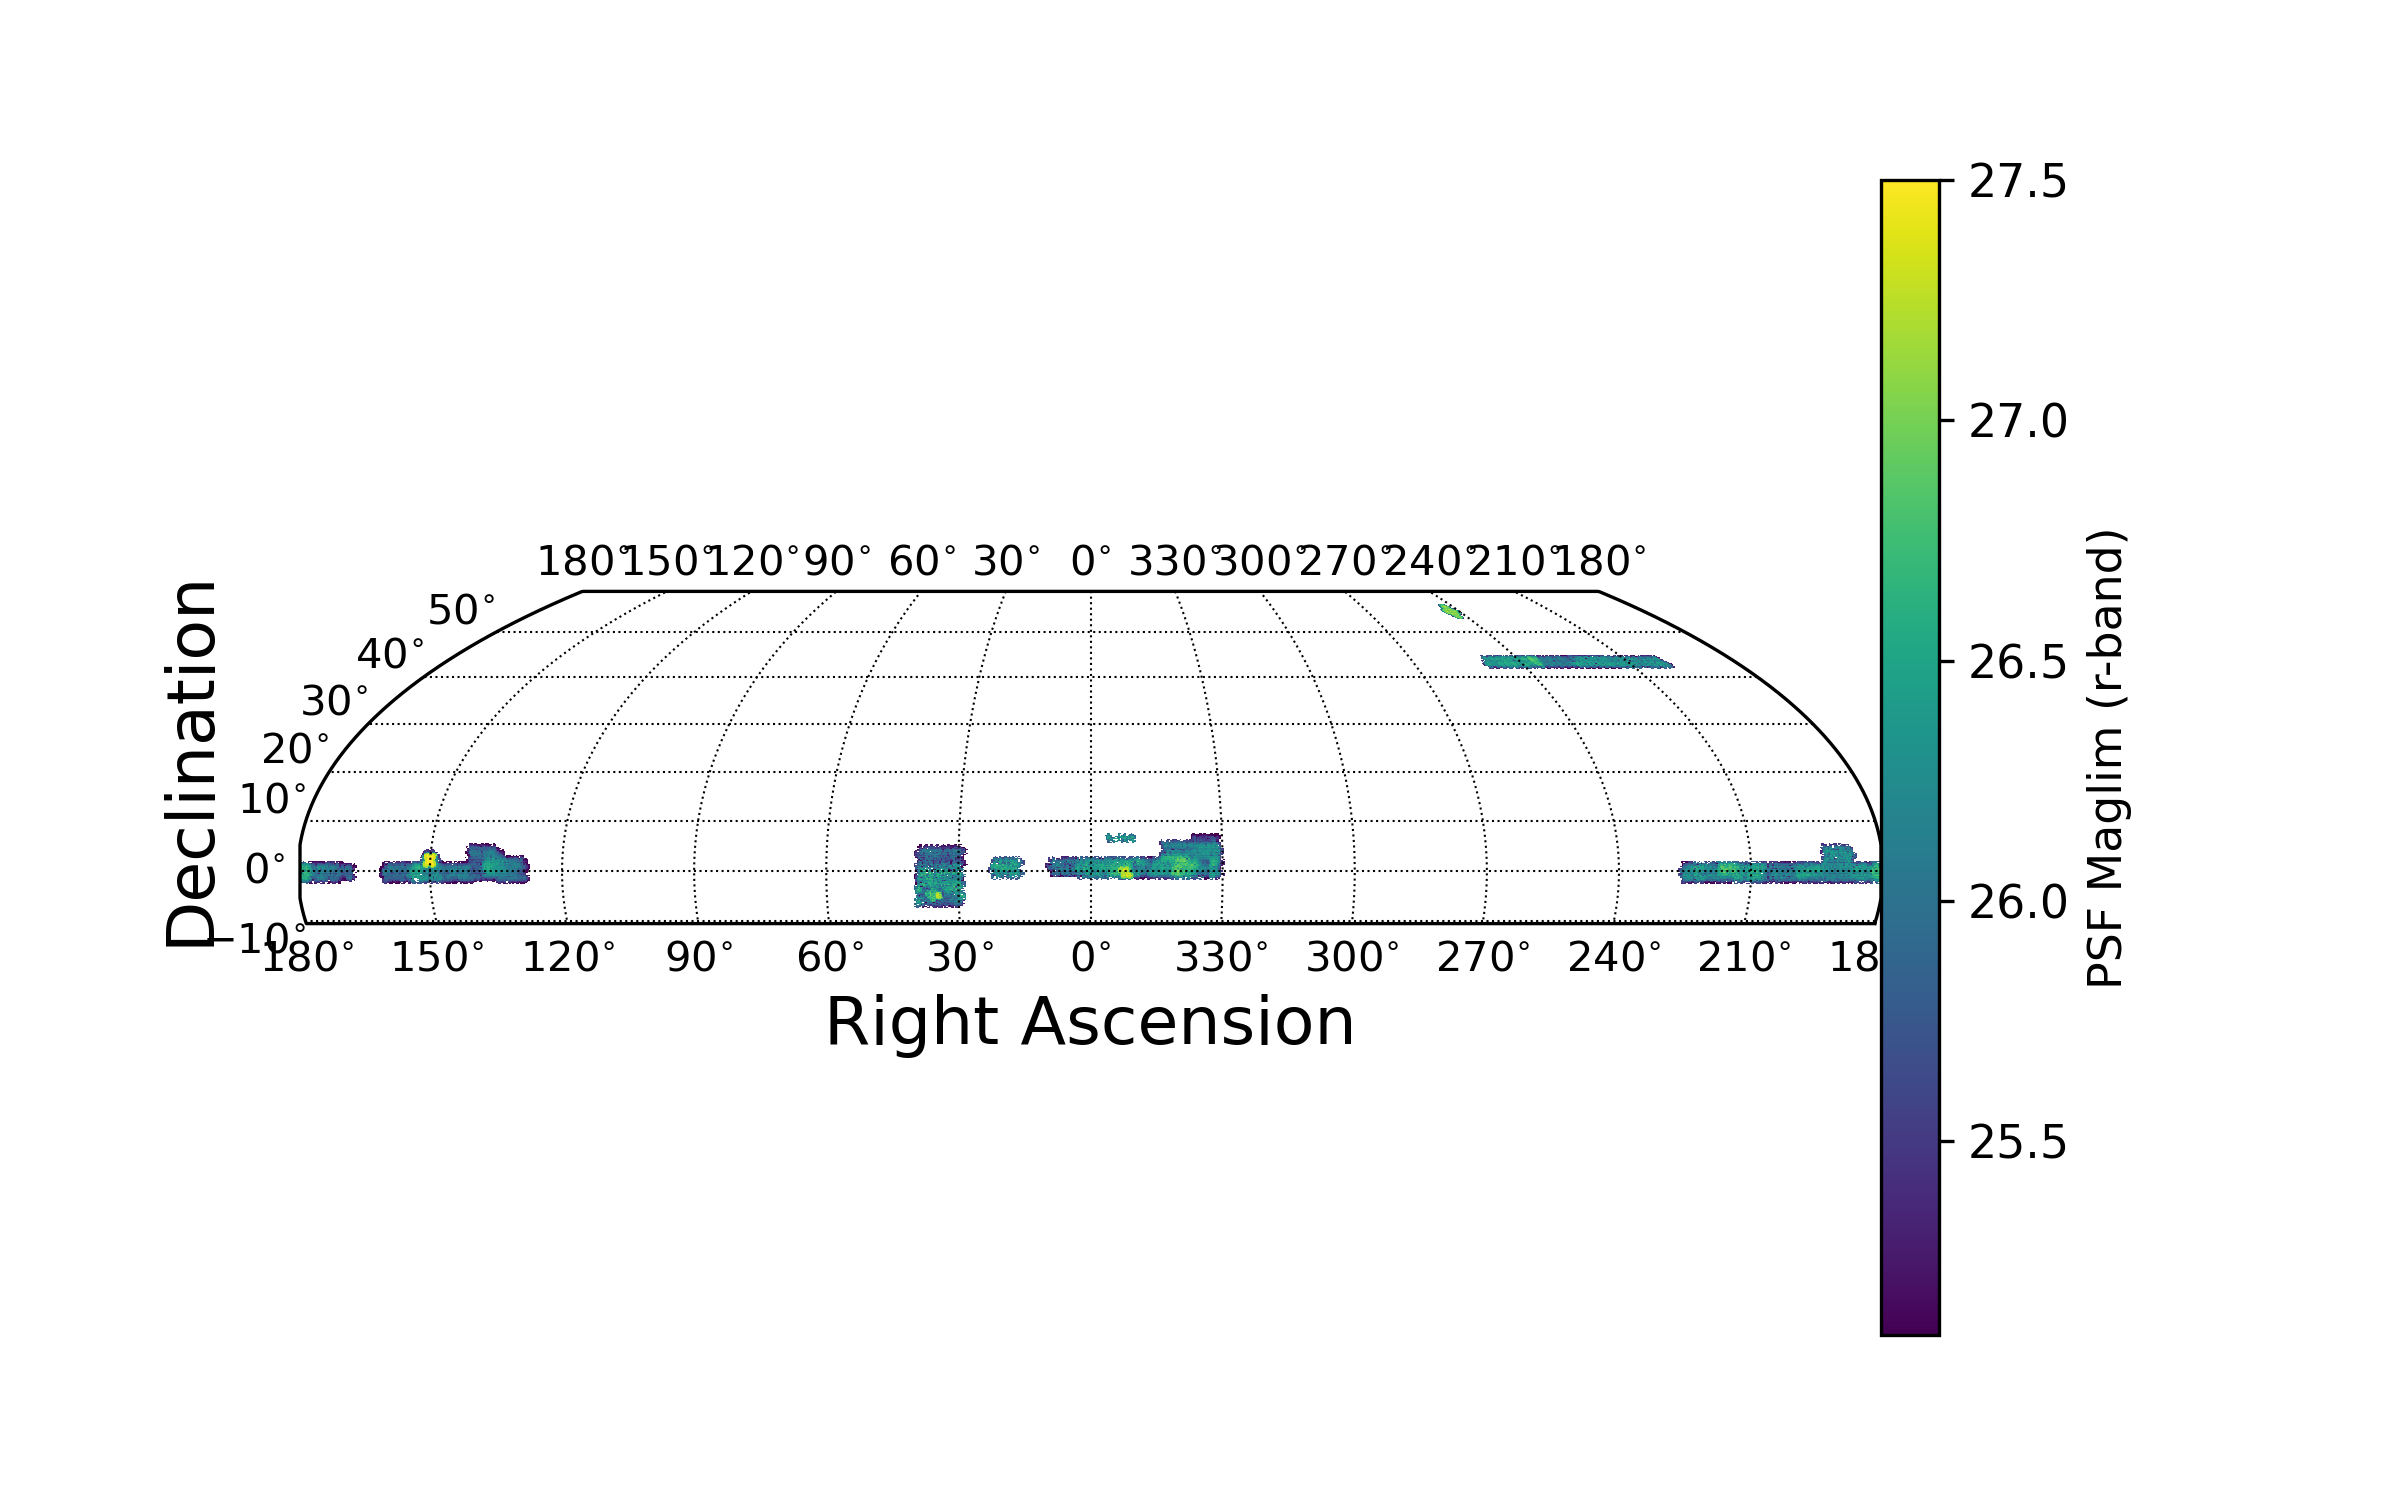
\includegraphics[width=0.9\textwidth]{r_maglim_pdr2.png}
	 \caption{Footprint of PDR2 processed dataset in equatorial coordinates.  \label{fig:footprint1}}
\end{figure}

 \begin{figure}[h]
 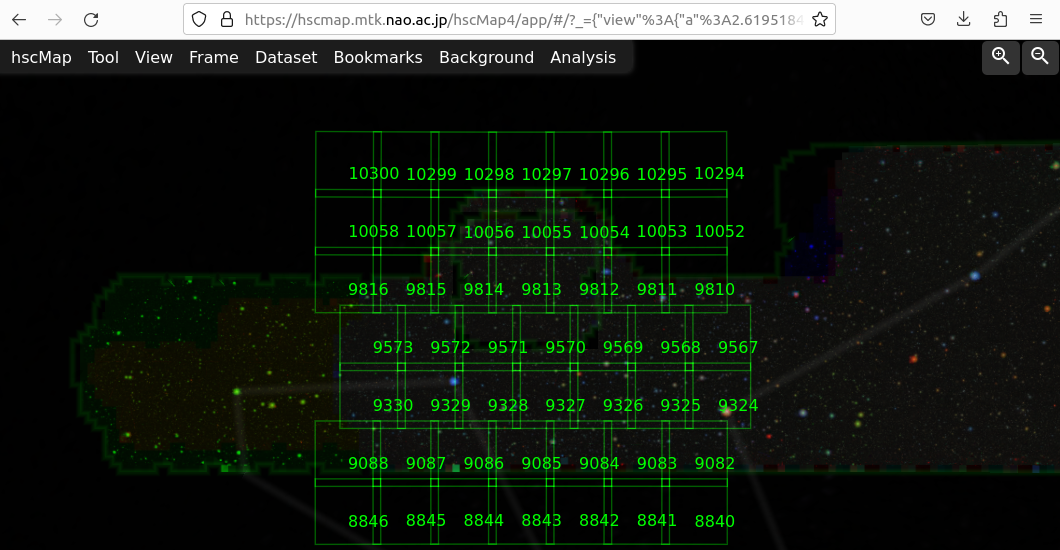
\includegraphics[width=0.9\textwidth]{hscmaptractcosmos.png}
	 \caption{PDR2 close up near COSMOS region (centered near $\rm (RA,DEC) = (150, 2)$ degrees), with tract numbers overlaid.  \label{fig:hscmaptract}}
 \end{figure}

\subsection{DRP processing overview and instrument comparison: HSC vs. LSSTCam}

Each detector is a 2K x 4K pixel CCD image, of size about 57MB.
There are 103 science quality CCDs/exposure.  Detector 9 is masked due
to known quality issues and ccds 104-112 are not on-sky science chips in
the HSC mosaic.

The HSC sky is divided into 'tracts' and each tract is subdivided 
into 'patches', as defined by the skymap ($\rm hsc\_rings\_v1$) which maps 
tract number to a square region in (RA,DEC) coordinates.

For HSC, each tract covers about 2.7 sq degrees on the sky and is
subdivided into 81 patches on a $9 \times 9$ grid.

In contrast, the full LSSTCam has 4K x 4K pixel CCDs, there are 
189 science CCDs each about 100 MB in size.  Furthermore each tract 
on the sky is divided into a $7\times 7$ grid of patches.

For purposes of this exercise, the calibration exposures (
flat fields in each band, biases, non-linearity maps, sky pupil per 
band, bad pixel, bad column,  gain and full well levels per amplifier) are 
all taken as given 'ancillary' inputs, pre-constructed and outside the
scope of this campaign.

For DP1, DP2 and DR1 all good visits obtained to over a certain time
interval, six months to one year in length are gathered at the
start of a DRP.  All raw exposures are processed through 
step1 (which consists of pipetasks for Instrument Signature 
Reduction (ISR), image and PSF characterization, source detection 
and measurement), 
step2a (combine gather source tables), and step2b (perform 
astrometric calibration with a 2MASS or eventually Gaia reference catalog,
extract calibration star catalogs) 
at multiple processing sites if available.  Each visit or detector may 
be processed independently (and many in parallel) 
for steps 1, 2a and 2b.

For the PDR2 HSC exercise, multi-site processing was not yet up, 
and so all processing was done at one site (the USDF at SLAC).

Following step2b, the extracted, (and relatively small),
calibration star catalogs are gathered together over the entire campaign
footprint and are used in step2c to generate a single Forward 
Global Calibration Module (FGCM) photometric solution with zeropoints for
each exposure processed.

These astrometric solutions and photometric zeropoints from steps 2b and 2c
respectively are applied in step2d and gathered together by visit in step2e.

There may be (and in the case of PDR2 there was) a 'visit-veto list' of 
poor quality (i.e. bad seeing) exposures identified at the end of step2e but 
prior to the start of step3.  A subcollection is made containing only 
the remaining good visits, which are used for further processing.  

For the HSC PDR2 case, about 2.5K out of 17.3K visits were rejected 
leaving about 15K visits to be coadded.

Step3 of PDR processing performs coaddition, combining all calibrated 
visit images, first 'warping' them using the astrometric solution to put 
them onto a common geometric footprint and then coadding them weighted 
appropriately by photometric flux zeropoint and noise properties.

The astrometric algorithm used for PDR2 HSC is called 'jointcal'.  This
older algorithm may be replaced by 'gbdes' in future processings, as that
algorithm accounts for 'tree rings', DCR 
(Differential Chromatic Refraction) and other subtle distortions \jira{DM-39933}.

Coadds for the HSC PDR2 footprint are currently done patch-by-patch,
though future processings will also produce 'overlapping cell-based' 
coadds \jira{DM-32345} which further subdivides patches and tracts into regions of 
the sky where the PSF in each band is well-modeled as constant 
across an entire cell with no discontinuous jumps due to detector edges.
These cell-based coadds in turn will allow for the accurate measurement of 
weak lensing shears of all source stacked objects when combined with
a PIFF PSF model.

Between May 2023 and (approx) Sep 2023 the HSC PDR2 was reprocessed with 
Rubin Science pipelines stack version v24.1.0, which was 
based on a weekly stack $\rm w\_2023\_11$.  Some modifications or fixes 
to the stack were applied during the processing, as described below.

In the sections that follow, we discuss campaign 
management \secref{sec:management}, 
processing \secref{sec:processing} and quality 
assurance \secref{sec:qa} details of the HSC PDR2 campaign.


